\chapauthor{Орлов М.К.\\Шункевич Д.В.\\Ковалёв М.В.\\Садовский М.Е.\\Загорский А.Г.\\Банцевич К.А.}
\chapter{Комплексная библиотека многократно используемых семантически совместимых компонентов ostis-систем}
\chapauthortoc{Орлов М.К.\\Шункевич Д.В.\\Ковалёв М.В.\\Садовский М.Е.\\Загорский А.Г.\\Банцевич К.А.}
\label{chapter_library}

\abstract{Важнейшим этапом эволюции любой технологии является переход к компонентному проектированию на основе постоянно пополняемый библиотеки многократно используемых компонентов. Идея библиотеки компонентов не нова, но семантическая мощность \scnkeyword{Библиотеки OSTIS} значительно выше аналогов за счет того, что подавляющее большинство компонентов библиотеки -- компоненты базы знаний, представленные на унифицированном языке представления знаний (\textit{SC-коде}). Таким образом, в \scnkeyword{Библиотеке OSTIS} обеспечивается высокий уровень семантической совместимости компонентов, что приводит к высокому уровню семантической совместимости ostis-систем, использующих библиотеку многократно используемых компонентов ostis-систем.}

\section{Структура комплексной библиотеки многократно используемых семантически совместимых компонентов ostis-систем}

Основной тезис - всё, что можно сделать одинаково, нужно делать одинаково.

% Зачем всё это надо
Повторное использование готовых компонентов широко применяется во многих отраслях, связанных с проектированием различного рода систем, поскольку позволяет уменьшить трудоемкость разработки и ее стоимость (путем минимизации количества труда за счет отсутствия необходимости разрабатывать какой-либо компонент), повысить качество создаваемого контента и снизить профессиональные требования к разработчикам компьютерных систем. Таким образом, осуществляется переход от программирования компонентов или целых систем к их дизайну на основе готовых компонентов. Использование готовых компонентов предполагает, что распространяемый компонент верифицирован и документирован, а возможные ошибки и ограничения устранены либо специфицированы и известны.

% Что мешает реализации того, что надо
В реализации компонентного подхода к проектированию интеллектуальных систем существуют следующие проблемы:
\begin{itemize}
	\item{Несовместимость компонентов, разработанных в рамках разных проектов, вследствие отсутствия унификации в принципах представления различных видов знаний в рамках одной базы знаний, и, как следствие, отсутствие унификации в принципах выделения и спецификации многократно используемых компонентов.}
	\item{Невозможность автоматической интеграции компонентов в систему без ручного вмешательства пользователя.}
	\item{Не ведётся разработка стандартов, обеспечивающих совместимость этих компонентов.}
	\item{Многие компоненты используют для идентификации язык разработчика (как правило, английский), и предполагается, что все пользователи будут использовать этот же язык. Однако для многих приложений это недопустимо – понятные только разработчику идентификаторы должны быть скрыты от конечных пользователей, которые должны быть в состоянии выбрать язык для идентификаторов, которые они видят}
	\item{Отсутствие средств поиска компонентов, удовлетворяющих заданных критериям.}
\end{itemize}

% Как обойти то, что мешает реализации того, что надо
Для того, чтобы решить возникшие проблемы, при проектировании интеллектуальных систем и библиотек их многократно используемых компонентов необходимо выполнить следующие требования:
\begin{itemize}
	\item{Использование универсального языка представления знаний, используемого в интеллектуальной системе.}
	\item{Наличие универсальной процедуры интеграции знаний в рамках указанного языка.}
	\item{Наличие стандарта, обеспечивающего семантическую совместимость интегрируемых знаний (таким стандартом является согласованная система используемых понятий).}
\end{itemize}

% Зачем это надо Технологии OSTIS
Основным требованием, предъявляемым к \textit{Технологии OSTIS}, является обеспечение возможности совместного использования в рамках ostis-систем различных \textit{видов знаний} и различных \textit{моделей решения задач} с возможностью \uline{неограниченного} расширения перечня используемых в ostis-системе видов знаний и моделей решения задач без существенных трудозатрат. Следствием данного требования является необходимость реализации компонентного подхода на всех уровнях, от простых компонентов баз знаний и решателей задач до целых ostis-систем.
Основу для реализации компонентного подхода в рамках \textit{Технологии OSTIS} составляет \scnkeyword{Библиотека OSTIS}. \textit{Метасистема OSTIS} ориентирована на разработку и практическое внедрение методов и средств компонентного проектирования семантически совместимых интеллектуальных систем, которая предоставляет возможность быстрого создания интеллектуальных систем различного назначения. В состав Метасистемы OSTIS входит \scnkeyword{Библиотека Метасистемы OSTIS}.
Сферы практического применения технологии компонентного проектирования семантически совместимых интеллектуальных систем ничем не ограничены.

% Понятие ябиблиотеки OSTIS
\begin{SCn}
	\scnheader{библиотека многократно используемых компонентов ostis-систем}
	\scntext{сокращение}{библиотека ostis-систем}
	\scnidtf{библиотека многократно используемых компонентов OSTIS}
	\scnhaselementrole{типичный пример}{\scnkeyword{Библиотека OSTIS}}
	\begin{scnindent}
		\scnidtf{Библиотека многократно используемых компонентов ostis-систем в составе Метасистемы OSTIS}
		\scnidtf{Библиотека Метасистемы OSTIS}
	\end{scnindent}
	\begin{scnreltoset}{объединение}
		\scnitem{библиотека типовых подсистем ostis-систем}
		\scnitem{библиотека шаблонов типовых компонентов ostis-систем}
		\scnitem{библиотека ostis-платформ}
		\scnitem{библиотека многократно используемых компонентов баз знаний}
		\scnitem{библиотека многократно используемых компонентов решателей задач}
		\scnitem{библиотека многократно используемых компонентов пользовательских интерфейсов}
	\end{scnreltoset}
\end{SCn}

% Зачем нужна Библиотека OSTIS
Основное назначение Библиотеки OSTIS -- создание условий для эффективного, осмысленного и массового проектирования ostis-систем и их компонентов путём создания среды для накопления и совместного использования компонентов ostis-систем. Такие условия осуществляются путём неограниченного расширения постоянно эволюционируемых семантически совместимых ostis-систем и их компонентов, входящих в \textit{Экосистему OSTIS}.

% Обоснование Библиотеки OSTIS для БЗ и РЗ
На сегодняшний день разработано большое число \textit{баз знаний} по самым различным предметным областям. Однако в большинстве случаев каждая база знаний разрабатывается отдельно и независимо от других, в отсутствие единой унифицированной формальной основы для представления знаний, а также единых принципов формирования систем понятий для описываемой предметной области. В связи с этим разработанные базы оказываются, как правило, несовместимы между собой и не пригодны для повторного использования. Компонентный подход к разработке интеллектуальных компьютерных систем, реализуемый в виде \scnkeyword{библиотеки многокртно используемых компонентов ostis-систем}, позволяет решить описанные проблемы.
В области разработки \textit{решателей задач} также существует большое количество конкретных реализаций, однако вопросы совместимости различных решателей при решении одной задачи практически не рассматриваются. Гипотетически возможно существование универсального решателя задач, объединяющего в себе все известные способы и методы решения задач. Однако использование такого решателя в прикладных целях не является целесообразным. Таким образом, наиболее приемлемым вариантом становится создание библиотеки совместимых между собой компонентов, из которых впоследствии может быть скомпилирован решатель, удовлетворяющий необходимым требованиям.
% TODO: написать про интерфейсы

Постоянно расширяемая Библиотека OSTIS существенно сокращает сроки разработки новых интеллектуальных компьютерных систем.
Библиотека ostis-систем позволяет избавиться от дублирования семантически эквивалентных информационных компонентов. А также от многообразия форм технической реализации используемых моделей решения задач.

% Что умеет библиотека ostis-систем
Функциональрные возможности библиотеки многократно используемых компонентов ostis-систем:
\begin{itemize}
	\item{Хранение многократно используемых компонентов ostis-систем и их спецификаций. При этом часть компонентов, специфицированных в рамках библиотеки, могут физически храниться в другом месте ввиду особенностей их  технической реализации (например, исходные тексты ostis-платформы могут физически храниться в каком-либо отдельном репозитории, но специфицированы как компонент будут в соответствующей библиотеке). В этом случае спецификация компонента в рамках библиотеки должна также включать описание (1) того где располагается компонент и (2) сценария его автоматической установки в дочернюю ostis-систему.}
	\item{Просмотр имеющихся компонентов и их спецификаций, а также поиск компонентов по фрагментам их спецификации.}
	\item{Хранение сведений о том, в каких ostis-системах-потребителях какие из компонентов библиотеки и какой версии используются (были скачаны). Это необходимо как минимум для учета востребованности того или иного компонента, оценки его важности и популярности.}
	\item{Систематизация многократно используемых компонентов ostis-систем.}
	\item{Обеспечение версионирования многократно используемых компонентов ostis-систем.}
	\item{Поиск зависимостей между многократно используемыми компонентами в рамках библиотеки компонентов.}
	\item{Формирование отдельных фрагментов многократно используемых компонентов ostis-систем.}
	\item{Обеспечение автоматического обновления компонентов, заимствованных в дочерние ostis-системы. Данная функция может включаться и отключаться по желанию разработчиков дочерней ostis-системы. Одновременное обновление одних и тех же компонентов во всех системах, его использующих, не должно ни в каком контексте приводить к несогласованности между этими системами. Это требование может оказаться довольно сложным, но без него работа Экосистемы OSTIS невозможна.}
\end{itemize}

\begin{SCn}
	\scnheader{библиотека многократно используемых компонентов ostis-систем}
	\begin{scnrelfromset}{обобщенная декомпозиция}
		\scnitem{база знаний библиотеки многократно используемых компонентов ostis-систем}
		\scnitem{решатель задач библиотеки многократно используемых компонентов ostis-систем}
		\scnitem{интерфейс библиотеки многократно используемых компонентов ostis-систем}
		\begin{scnindent}
			\begin{scnrelfromset}{декомпозиция}
				\scnitem{минимальный интерфейс библиотеки многократно используемых компонентов ostis-систем}
				\scnitem{расширенный интерфейс библиотеки многократно используемых компонентов ostis-систем}
				\begin{scnindent}
					\scnidtf{графический интерфейс библиотеки многократно используемых компонентов ostis-систем}
				\end{scnindent}
			\end{scnrelfromset}
		\end{scnindent}
	\end{scnrelfromset}
\end{SCn}

Решатель задач библиотеки многократно используемых компонентов ostis-систем реализует функциональные возможности библиотеки ostis-систем.

База знаний библиотеки мнoгократно используемых компонентов ostis-систем представляет собой иерархию многократно используемых компонентов ostis-систем и их спецификаций.

Интерфейс библиотеки ostis-систем обеспечивает доступ к многократно используемым компонентам и возможностям библиотеки ostis-систем для пользователя и других систем. Существует минимальный и расширенный интерфейс библиотеки многократно используемых компонентов ostis-систем. Минимальный интерфейс позволяет \textit{менеджеру многократно используемых компонентов ostis-систем}, входящему в состав какой-либо дочерней ostis-системы, подключиться к библиотеке многократно используемых компонентов ostis-систем и использовать ее функциональные возможности, то есть, например, получить доступ к спецификации компонентов и установить выбранные компоненты в дочернюю ostis-систему, получить сведения до доступных версиях компонента, его зависимостях и т.д. Расширенный интерфейс, в отличие от минимального интерфейса, позволяет не только получить доступ к компонентам для дальнейшей работы с ними, но и просматривать существующую структуру библиотеки,  а также компоненты и их элементы в удобном и интуитивно понятном для пользователя виде.

% Как подключить библиотеку ostis-систем. Иерархие материнских и дочерних систем
Разработчики \uline{любой} \textit{ostis-системы} могут включить в ее состав библиотеку, которая позволит им накапливать и распространять результаты своей деятельности среди других участников \textit{Экосистемы OSTIS} в виде \scnkeyword{многократно используемых компонентов}. Решение о включении компонента в библиотеку принимается экспертным сообществом разработчиков, ответственным за качество этой библиотеки. Верификацию компонентов можно автоматизировать.
В рамках \textit{Экосистемы OSTIS} существует множество библиотек многократно используемых компонентов ostis-систем, являющихся подсистемами соответствующих материнских ostis-систем. Главной библиотекой многократно используемых компонентов ostis-систем является \textit{Библиотека Метасистемы OSTIS}. \textit{Метасистема OSTIS} выступает \scnkeyword{материнской системой} для всех разрабатываемых ostis-систем, поскольку содержит все базовые компоненты (рисунок \textit{\nameref{fig:ecosystem_architecture}}). Материнская система отвечает за какой-то класс компонентов и является САПРом для этого класса, содержит методики разработки таких компонентов, их классификацию, подробные пояснения ко всем подклассам компонентов. Таким образом, формируется иерархия \scnkeyword{материнских ostis-систем}. Материнская ostis-система в свою очередь может являться дочерней ostis-системой для какой-либо другой ostis-системы, заимствуя компоненты из библиотеки, входящей в состав этой другой ostis-системы.

\begin{SCn}
\scnheader{ostis-система}
\scnsuperset{материнская ostis-система}
\begin{scnindent}
	\scnidtf{ostis-система, имеющая в своем составе библиотеку многократно используемых компонентов.}
	\scnhaselement{Метасистема OSTIS}
\end{scnindent}
\scnsuperset{дочерняя ostis-система}
\begin{scnindent}
	\scnidtf{ostis-система, в составе которой имеется компонент, заимствованный из какой-либо библиотеки многократно используемых компонентов.}
\end{scnindent}
\end{SCn}


\begin{figure}[H]
	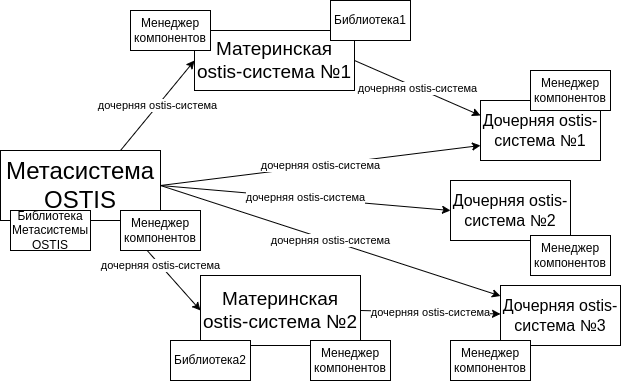
\includegraphics[scale=0.8]{author/part5/figures/ecosystem_architecture.png}
	\caption{Архитектура Экосистемы OSTIS}
	\label{fig:ecosystem_architecture}
\end{figure}

% Как происходит интеграция компонентов. Перенести выше?
Интеграция многократно используемых компонентов ostis-систем сводится к склеиванию ключевых узлов по идентификаторам и устранению	возможных дублирований и противоречий исходя из спецификации компонента и его содержания. Интеграция любых компонентов ostis-систем происходит автоматически, без вмешательства разработчика. Это достигается за счёт использования \textit{SC-кода} и его преимуществ, унификации спецификации многократно используемых компонентов и тщательного отбора компонентов в библиотеках экспертным сообществом, ответственным за эту библиотеку.

% Понятие многократно используемого компонента ostis-систем
Под многократно используемым компонентом ostis-систем понимается  компонент некоторой ostis-системы, который может быть использован в рамках другой ostis-системы. Это компонент ostis-системы, который может быть использован в других ostis-системах (\scnkeyword{дочерних ostis-системах}) и содержит все те и только те sc-элементы, которые необходимы для функционирования компонента в дочерней ostis-системе. Другими словами это компонент некоторой \scnkeyword{материнской ostis-системы}, который может быть использован в некоторой \scnkeyword{дочерней ostis-системе}. Многократно используемые компоненты должны иметь унифицированную спецификацию и иерархию для поддержки \uline{совместимости} с другими компонентами. Совместимость многократно используемых компонентов приводит систему к новому качеству, к дополнительному расширению множества решаемых задач при интеграции компонентов.

\begin{SCn}
	\scnheader{многократно используемый компонент ostis-систем}
	\scnidtf{многократно используемый компонент OSTIS}
	\scnidtftext{часто используемый sc-идентификатор}{многократно используемый компонент}
	\scnsubset{компонент ostis-системы}
\end{SCn}

Компонент ostis-системы -- это целостная часть ostis-системы, которая содержит все те (и только те) sc-элементы, которые необходимы для её функционирования в ostis-системе.
Отличие многократно используемого компонента ostis-систем от компонента ostis-системы в том, что многократно используемый компонент имеет \uline{спецификацию, достаточную для установки} этого компонента в \scnkeyword{дочернюю ostis-систему}. Спецификация является частью базы знаний \scnkeyword{библиотеки многократно используемых компонентов} соответствующей \scnkeyword{материнской ostis-системы}. Есть техническая возможность встроить многократно используемый компонент в дочернюю ostis-систему.

Необходимые требования, предъявляемые к многократно используемым компонентам ostis-истем:
\begin{itemize}
	\item{Существует техническая возможность встроить многократно используемый компонент в \scnkeyword{дочернюю ostis-систему}.}
	\item{Полнота многократно используемого компонента: компонент должен в полной мере выполнять свои функции, соответствовать своему назначению.}
	\item{Связность многократно используемого компонента: компонент должен логически выполнять только одну задачу из предметной области, для которой он предназначен. Многократно используемый компонент должен выполнять свои функции наиболее общим образом, чтобы круг возможных систем, в которые он может быть встроен, был наиболее широким.}
	\item{Совместимость многократно используемого компонента: компонент должен стремиться повышать уровень \uline{договороспособности} ostis-систем, в которые он встроен и иметь возможность \uline{автоматической} интеграции в другие системы;}
	% Это уточнение полоны? Или связности
	\item{Самодостаточность компонентов (или групп компонентов) технологии, т.е. способности их функционировать отдельно от других компонентов без утраты целесообразности их использования.}
\end{itemize}

% Классификация многократно используемых компонентов ostis-систем
Рассмотрим классификацию многократно используемых компонентов ostis-систем. Класс многократно используемого компонента ostis-систем является важной частью спецификации компонента, позволяющей лучше понять назначение и область применения данного компонента, а также класс многократно используемого компонента является важнейшим критерием поиска компонентов в библиотеке ostis-систем. Основной признак классификации многократно используемых компонентов является признак предметной области, к которой относится компонент. Здесь структура может быть довольно богатой в соответствии с иерархией областей человеческой деятельности.

\begin{SCn}	
\scnheader{многократно используемый компонент ostis-систем}
\begin{scnrelfromset}{разбиение}
	\scnitem{многократно используемый компонент базы знаний}
	\begin{scnindent}
		\scnsuperset{семантическая окрестность}
		\scnsuperset{предметная область и онтология}
		\scnsuperset{база знаний}
		\scnsuperset{шаблон типового компонента ostis-систем}
		\begin{scnindent}
			\scnhaselement{Шаблон описания sc-модели предметной области}
			\scnhaselement{Шаблон описания отношения}
		\end{scnindent}
	\end{scnindent}
	\scnitem{многократно используемый компонент решателя задач}
	\begin{scnindent}
		\scnsuperset{атомарный агент обработки знаний}
		\scnsuperset{программа обработки знаний}
	\end{scnindent}
	\scnitem{многократно используемый компонент интерфейса}
	\begin{scnindent}
		\scnsuperset{многократно используемйы компонент пользовательского интерфейса для отображения}
		\scnsuperset{интерактивный многократно используемый компонент пользовательского интерфейса}
	\end{scnindent}
\end{scnrelfromset}
\end{SCn}	

Для компонентов баз знаний важнейшим признаком классификации многократно используемых компонентов является вид используемых знаний. Для компонентов решателя задач - модель решения задач. Для компонентов интерфейса - вид интерфейса в соответствии с классификацией компонентов пользовательских интерфейсов.

\begin{SCn}	
\scnheader{многократно используемый компонент ostis-систем}
\scnrelfrom{разбиение}{\scnkeyword{Типология компонентов ostis-систем по атомарности\scnsupergroupsign}}
\begin{scnindent}
	\begin{scneqtoset}
		\scnitem{атомарный многократно используемый компонент ostis-систем}
		\scnitem{неатомарный многократно используемый компонент ostis-систем}
	\end{scneqtoset}
\end{scnindent}
\end{SCn}

Атомарный многократно используемый компонент ostis-систем -- это компонент, который в текущем состоянии библиотеки ostis-систем рассматривается как неделимый, то есть не содержит в своем составе других компонентов. Принадлежность многократно используемого компонента ostis-систем классу атомарных компонентов зависит от того, как специфицирован этот компонент и от существующих на данный момент компонентов в библиотеке. Неатомарный многократно используемый компонент в текущем состоянии библиотеки ostis-систем содержит в своем составе другие атомарные или неатомарные компоненты, он не зависит от своих частей. Без какой-либо части неатомарного компонента его назначение сужается. В общем случае атомарный компонент может перейти в разряд неатомарных в случае, если будет принято решение выделить какую-то из его частей в качестве отдельного компонента. Все вышесказанное, однако, не означает, что даже в случае его платформенной независимости, атомарный компонент всегда хранится в sc-памяти как сформированная sc-структура. Например, платформенно-независимая реализация sc-агента всегда будет представлена набором scp-программ, но будет атомарным многократно используемым компонентом OSTIS в случае, если ни одна из этих
программ не будет представлять интереса как самостоятельный компонент. В общем случае неатомарный компонент может перейти в разряд атомарных в случае, если будет принято решение по каким-либо причинам исключить все его части из рассмотрения в качестве отдельных компонентов. Следует отметить, что неатомарный компонент необязательно должен складываться полностью из других компонентов, в его состав могут также входить и части, не являющиеся самостоятельными компонентами. Например, в состав реализованного
на языке SCP sc-агента, являющего неатомарным многократно используемым компонентом могут входить как scp-программы, которые могут являться многократно используемыми компонентами (а могут и не являться), а также агентная scp-программа, которая не имеет смысла как многократно используемый компонент.

\begin{SCn}	
\scnheader{многократно используемый компонент ostis-систем}
\scnrelfrom{разбиение}{\scnkeyword{Типология компонентов ostis-систем по зависимости\scnsupergroupsign}}
\begin{scnindent}
	\begin{scneqtoset}
		\scnitem{зависимый многократно используемый компонент ostis-систем}
		\scnitem{независимый многократно используемый компонент ostis-систем}
	\end{scneqtoset}
\end{scnindent}
\end{SCn}

% Кличко talks
Зависимый многократно используемый компонент ostis-систем зависит хотя бы от одного другого компонента библиотеки ostis-систем, т.е. не может быть встроен в дочернюю ostis-систему без компонентов, от которых он зависит. Независимый компонент не зависит ни от одного другого компонента библиотеки ostis-систем.

\begin{SCn}
\scnheader{многократно используемый компонент ostis-систем}
\scnrelfrom{разбиение}{\scnkeyword{Типология компонентов ostis-систем по способу их хранения\scnsupergroupsign}}
\begin{scnindent}
	\begin{scneqtoset}
		\scnitem{многократно используемый компонент ostis-систем, хранящийся в виде внешних файлов}
		\begin{scnindent}
			\begin{scnrelfromset}{разбиение}
				\scnitem{многократно используемый компонент ostis-систем, хранящийся в виде файлов исходных текстов}
				\scnitem{многократно используемый компонент ostis-систем, хранящийся в виде скомпилированных файлов}
			\end{scnrelfromset}
		\end{scnindent}
		\scnitem{многократно используемый компонент, хранящийся в виде sc-структуры}
	\end{scneqtoset}
\end{scnindent}
\end{SCn}

На данном этапе развития \textit{Технологии OSTIS} более удобным является хранение компонентов в виде исходных текстов.

\begin{SCn}
\scnheader{многократно используемый компонент ostis-систем}
\scnrelfrom{разбиение}{\scnkeyword{Типология компонентов ostis-систем по зависимости от ostis-платформы\scnsupergroupsign}}
\begin{scnindent}
	\begin{scneqtoset}
		\scnitem{платформенно-зависимый многократно используемый компонент ostis-систем}
		\begin{scnindent}
			\scnsuperset{ostis-платформа}
			\scnsuperset{абстрактный sc-агент, не реализуемый на Языке SCP}
		\end{scnindent}
		\scnitem{платформенно-независимый многократно используемый компонент ostis-систем}
		\begin{scnindent}
			\scnsuperset{многократно используемый компонент базы знаний}
			\scnsuperset{SCP-агент}
			\scnsuperset{SCP-программа}
		\end{scnindent}
	\end{scneqtoset}
\end{scnindent}
\end{SCn}

Под платформенно-зависимым многократно используемым компонентом ostis-систем понимается компонент, частично или полностью реализованный при помощи каких-либо сторонних с точки зрения \textit{Технологии OSTIS} средств. Недостаток таких компонентов в том, что интеграция таких компонентов в интеллектуальные системы может сопровождаться дополнительными трудностями, зависящими от конкретных средств реализации компонента. В качестве возможного преимущества платформенно-зависимых многократно используемых компонентов ostis-систем
можно выделить их, как правило, более высокую производительность за счет реализации их на более приближенном к платформе уровне. В общем случае платформенно-зависимый многократно используемый компонент ostis-систем может поставляться как в виде набора исходных кодов, так и скомпилированном виде. Процесс интеграции платформенно-зависимого
многократно используемого компонента ostis-систем в дочернюю систему, разработанную по Технологии OSTIS, сильно зависит от технологий реализации данного компонента и в каждом конкретном случае может состоять из различных этапов. Каждый платформенно-зависимый многократно используемый компонент ostis-систем должен иметь соответствующую подробную, корректную и понятную инструкцию по его установке и внедрению в дочернюю систему.
Под платформенно-независимым многократно используемым компонентом ostis-систем понимается компонент, который целиком и полностью представлен на \textit{SC-коде}. В случае неатомарного многократно используемого компонента это означает, что все более простые компоненты, входящие в его состав также обязаны быть платформенно-независимыми многократно используемыми компонентами ostis-систем. Процесс интеграции платформенно-зависимого многократно используемого компонента ostis-систем в дочернюю систему, разработанную по Технологии OSTIS, существенно упрощается за счет использования общей унифицированной
формальной основы представления и обработки знаний.

Наиболее ценными являются платформенно-независимые многократно используемые компоненты ostis-систем.

\begin{SCn}
\scnheader{многократно используемый компонент ostis-систем}
\scnrelfrom{разбиение}{\scnkeyword{Типология компонентов ostis-систем по динамичности их установки\scnsupergroupsign}}
\begin{scnindent}
	\begin{scneqtoset}
		\scnitem{динамически устанавливаемый многократно используемый компонент ostis-систем}
		\begin{scnindent}
			\scnidtf{многократно используемый компонент, при установке которого система не требует перезапуска}
			\begin{scnrelfromset}{декомпозиция}
				\scnitem{многократно используемый компонент, хранящийся в виде скомпилированных файлов}
				\scnitem{многократно используемый компонент базы знаний}
			\end{scnrelfromset}
		\end{scnindent}
		\scnitem{многократно используемый компонент, при установке которого система требует перезапуска}
	\end{scneqtoset}
\end{scnindent}
\end{SCn}

Процесс интеграции компонентов разных видов на разных этапах жизненного цикла osits-систем бывает разным. Наиболее ценными являются компоненты, которые могут быть интегрированы в работающую систему \uline{без} прекращения её функционирования. Некоторые системы, особенно системы управления, нельзя останавливать, а устанавливать и обновлять компоненты нужно.

\begin{SCn}
\scnheader{многократно используемый компонент ostis-систем}
\scnsuperset{типовая подсистема ostis-систем}
\begin{scnindent}
	\scnhaselement{Среда коллективной разработки баз знаний ostis-систем}
	\scnhaselement{Визуальный web-ориентированный редактор sc.g-текстов}
\end{scnindent}
\end{SCn}

% Хранилище компонентов
Для того, чтобы хранить многократно используеме компоненты ostis-систем, необходимо некоторое хранилище. Таким хранилищем может выступать как какая-либо ostis-система, так и сторонее хранилище, например, облачный сервис. Помимо внешних файлов компонента в хранилище должна находиться его \uline{спецификация}.

% Спецификация многократно используемых компонентов
Каждый \textit{многократно используемый компонент ostis-систем} должен быть специфицирован в рамках библиотеки. Данные спецификации включают в себя основные знания о компоненте, которые позволяют обеспечить построение полной иерархии компонентов и их зависимостей, а также обеспечивают \uline{беспрепятственную} интеграцию компонентов в \scnkeyword{дочерние ostis-системы}. Для спецификации компонента используеются, как отношения, так и классы компонента.

Чтобы многократно используемый компонент мог быть принят в библиотеку, нужно специфицировать его используя \textit{необходимое для установки отношение, специфицирующее многократно используемый компонент ostis-систем}. В то же время \textit{необязательное для установки отношение, специфицирующее многократно используемый компонент ostis-систем} помогает лучше понять суть компонента, упрощает поиск, но не является обязательным для того, чтобы компонент мог быть установлен в ostis-систему.


\begin{SCn}
\scnheader{отношение, специфицирующее многократно используемый компонент ostis-систем\scnsupergroupsign}
\scnidtf{отношение, которое используется при спецификации многократно используемого компонента ostis-систем}
\begin{scnrelfromset}{разбиение}
	\scnitem{необходимое для установки отношение, специфицирующее многократно используемый компонент ostis-систем}
	\begin{scnindent}
		\scnhaselement{метод установки*}
		\scnhaselement{адрес хранилища*}
		\scnhaselement{зависимости компонента*}
	\end{scnindent}
	\scnitem{необязательное для установки отношение, специфицирующее многократно используемый компонент ostis-систем}
	\begin{scnindent}
		\scnhaselement{сопутствующий компонент*}
		\scnhaselement{история изменений*}
		\scnhaselement{авторы*}
		\scnhaselement{примечание*}
		\scnhaselement{пояснение*}
		\scnhaselement{идентификатор*}
		\scnhaselement{ключевой sc-элемент*}
		\scnhaselement{назначение*}
	\end{scnindent}
\end{scnrelfromset}
\end{SCn}

Метод установки позволяет пользователю установить компонент вручную, а \scnkeyword{менеджеру компонентов} - автоматически. Основные два метода установки многократно используемых компонентов - метод установки динамически устанавливаемого многократно используемого компонента ostis-систем и метод установки многократно используемого компонента, при установке которого система требует перезапуска. При динамической установке необходимо только скачать компонент, и он сразу же функционирует в системе. 

\begin{figure}[H]
	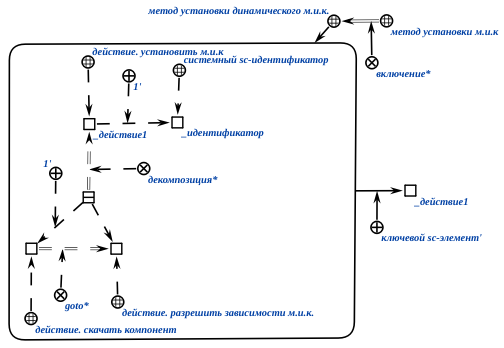
\includegraphics[scale=0.8]{author/part5/figures/install_dynamic_method.png}
	\caption{Метод установки динамически устанавливаемого многократно используемого компонента ostis-систем}
	\label{fig:dynamic_method}
\end{figure}

При установке компонента, при установке которого система требует перезапуска необходимо помимо скачивания компонента транслировать его в память системы.

\begin{figure}[H]
	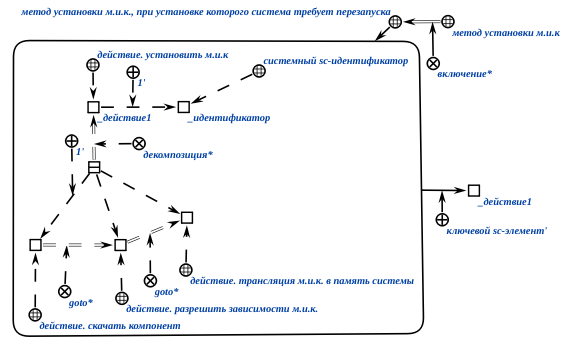
\includegraphics[scale=0.8]{author/part5/figures/install_with_reboot_method.png}
	\caption{Метод установки динамически устанавливаемого многократно используемого компонента, при установке которого система требует перезапуска}
	\label{fig:install_with_reboot_method}
\end{figure}


Связки отношения \textit{адрес хранилища*} связывают многократно используемый компонент, хранящийся в виде внешних файлов и файл, содержащий url-адрес многократно используемого компонента ostis-систем. Таким файлом может быть файл, содержащий url-адрес на GitHub многократно используемого компонента ostis-систем, файл, содержащий url-адрес на Google Drive многократно используемого компонента ostis-систем, файл, содержащий url-адрес на Docker Hub многократно используемого компонента ostis-систем и другие.

Связки отношения \textit{зависимости компонента*} связывают многократно используемый компонент, и множество компонентов, без которых устанавливаемый компонент \uline{не может быть} встроен в \scnkeyword{дочернюю ostis-систему}.

\begin{figure}[H]
	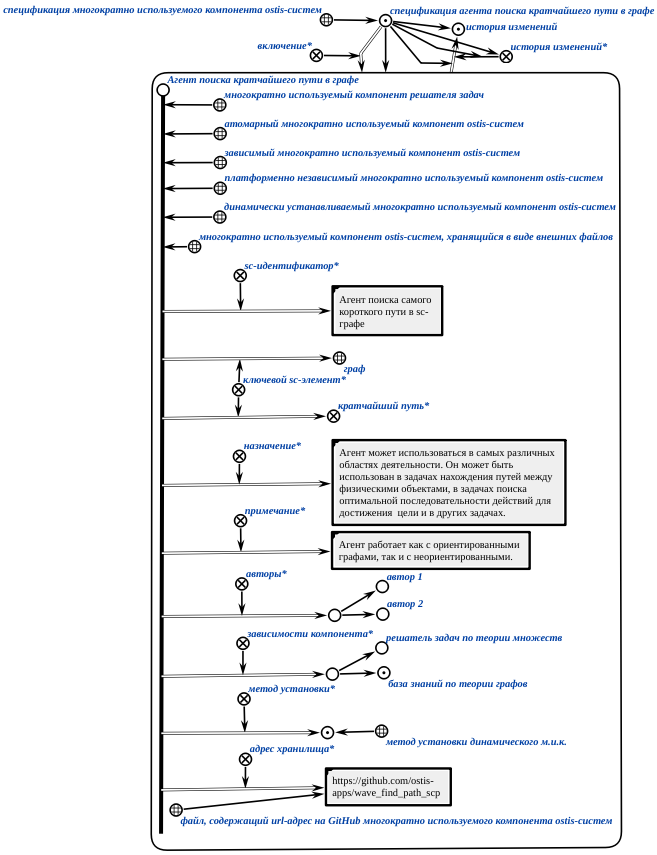
\includegraphics[scale=0.8]{author/part5/figures/component_specification_example.png}
	\caption{Пример спецификации многократно используемого компонента ostis-систем}
	\label{fig:component_specification_example}
\end{figure}

В некоторых случаях может оказаться, что для использования одного многократно используемого компонента OSTIS целесообразно или даже необходимо дополнительно использовать несколько других многократно используемых компонентов OSTIS. Например, может оказаться целесообразным вместе с каким либо sc-агентом информационного поиска использовать соответствующую команду интерфейса, которая представлена отдельным
компонентом и позволит пользователю задавать вопрос для указанного sc-агента через интерфейс системы. В таких случаях для связи компонентов используется отношение сопутствующий компонент*. Наличие таких связей позволяет устранить возможные проблемы неполноты знаний и навыков в дочерней системе, из-за которых какие-либо из компонентов могут не выполнять свои функции. Связки отношения сопутствующий компонент* связывают многократно используемые компоненты ostis-систем, которые целесообразно использовать в дочерней системе вместе. Каждая такая связка может дополнительно быть снабжена sc-комментарием или sc-пояснением, отражающим суть указываемой зависимости.

% Менеджер компонентов
Менеджер многократно используемых компонентов ostis-систем -- подсистема ostis-системы, с помощью которой проиходит взаимодействие с библиотекой компонентов ostis-систем.

\begin{SCn}
\scnheader{менеджер многократно используемых компонентов ostis-систем}
\scnidtftext{часто используемый sc-идентификатор}{менеджер многократно используемых компонентов}
\scnidtftext{часто используемый sc-идентификатор}{менеджер компонентов}
\begin{scnrelfromset}{обобщенная декомпозиция}
	\scnitem{база знаний менеджера многократно используемых компонентов ostis-систем}
	\scnitem{решатель задач менеджера многократно используемых компонентов ostis-систем}
	\scnitem{интерфейс менеджера многократно используемых компонентов ostis-систем}
\end{scnrelfromset}
\end{SCn}

База знаний менеджера компонентов содержит все те знания, которые необходимы для установки многократно используемого компонента в \scnkeyword{дочернюю ostis-систему}. К таким знаниям относятся знания о спецификации многократно используемых компонентов, методы установки компонентов, знание о  библиотеках ostis-систем, с которыми происходит взаимодействие. Решатель задач менеджера компонентов взаимодействует с библиотекой ostis-систем и позволяет установить и интегрировать многократно используемые компоненты в \scnkeyword{дочернюю ostis-систему}, также выполнять поиск, обновление, публикацию, удаление компонентов. Интерфейс менеджера многократно используемых компонентов обеспечивает удобное для пользователя и других систем использование менеджера компонентов.

Функциональные возможности менеджера компонентов ostis-систем следующие:
\begin{itemize}
	\item{\textbf{Поиск многократно используемых компонентов ostis-систем}. Множество возможных критериев поиска соответствует спецификации многократно используемых компонентов. Такими критериями могут быть классы компонента, его авторы, идентификатор, фрагмент примечания, назначение, принадлежность какой-либо предметной области, вид знаний компонента и другие.}
	\item{\textbf{Установка многократно используемого компонента ostis-систем}. Установка многократно используемого компонента происходит вне зависимости от типологии, способа установки и местоположения компонента. Необходимое условие для возможности установки многократно используемого компонента -- наличие \scnkeyword{спецификации многократно используемого компонента ostis-систем}. Перед установкой многократно используемого компонента в дочернюю систему необходимо разрешить все зависимости путём установки зависимых компонентов. После успешной установки компонента, в базе знаний дочерней системы генерируется информационная конструкция, обозначающая факт установки компонента в систему с помощью отношения \textit{установленные компоненты*}. После установки компонента в ostis-систему могут возникнуть противоречия в базе знаний, которые  устраняются с помощью средств обнаружения и анализа ошибок и противоречий в базе знаний ostis-системы.}
	\item{\textbf{Публикация многократно используемого компонента ostis-систем в библиотеку ostis-систем}. При публикации компонента в библиотеку ostis-систем происходит верификация на основе спецификации компонента. Также существует возможность обновления версии опубликованного компонента сообществом его разработчиков.}
	\item{\textbf{Обновление установленного многократно используемого компонента ostis-систем}}
	\item{\textbf{Удаление установленного многократно используемого компонента}. Как и в случае установки после удаления многократно используемого компонента из ostis-системы в базе знаний системы устанавливается факт удаления компонента. Эта информация является важной частью \uline{истории эксплуатации} ostis-системы.}
	\item{\textbf{Добавление и удаление отслеживаемых ostis-системой библиотек}. Менеджер компонентов содержит информацию о множестве источников для установки компонентов, перечень которых можно дополнять вручную. По умолчанию менеджер компонентов отслеживает Библиотеку Метасистемы OSTIS, однако можно создавать и добавлять дополнительные библиотеки ostis-систем.}
\end{itemize}

\section{Многократно используемые компоненты баз знаний ostis-систем}
\section{Многократно используемые встраиваемые ostis-системы}

%%%%%%%%%%%%%%%%%%%%%%%%% referenc.tex %%%%%%%%%%%%%%%%%%%%%%%%%%%%%%
% sample references
% %
% Use this file as a template for your own input.
%
%%%%%%%%%%%%%%%%%%%%%%%% Springer-Verlag %%%%%%%%%%%%%%%%%%%%%%%%%%
%
% BibTeX users please use
% \bibliographystyle{}
% \bibliography{}
%
\biblstarthook{In view of the parallel print and (chapter-wise) online publication of your book at \url{www.springerlink.com} it has been decided that -- as a genreral rule --  references should be sorted chapter-wise and placed at the end of the individual chapters. However, upon agreement with your contact at Springer you may list your references in a single seperate chapter at the end of your book. Deactivate the class option \texttt{sectrefs} and the \texttt{thebibliography} environment will be put out as a chapter of its own.\\\indent
References may be \textit{cited} in the text either by number (preferred) or by author/year.\footnote{Make sure that all references from the list are cited in the text. Those not cited should be moved to a separate \textit{Further Reading} section or chapter.} If the citatiion in the text is numbered, the reference list should be arranged in ascending order. If the citation in the text is author/year, the reference list should be \textit{sorted} alphabetically and if there are several works by the same author, the following order should be used:
\begin{enumerate}
\item all works by the author alone, ordered chronologically by year of publication
\item all works by the author with a coauthor, ordered alphabetically by coauthor
\item all works by the author with several coauthors, ordered chronologically by year of publication.
\end{enumerate}
The \textit{styling} of references\footnote{Always use the standard abbreviation of a journal's name according to the ISSN \textit{List of Title Word Abbreviations}, see \url{http://www.issn.org/en/node/344}} depends on the subject of your book:
\begin{itemize}
\item The \textit{two} recommended styles for references in books on \textit{mathematical, physical, statistical and computer sciences} are depicted in ~\cite{science-contrib, science-online, science-mono, science-journal, science-DOI} and ~\cite{phys-online, phys-mono, phys-journal, phys-DOI, phys-contrib}.
\item Examples of the most commonly used reference style in books on \textit{Psychology, Social Sciences} are~\cite{psysoc-mono, psysoc-online,psysoc-journal, psysoc-contrib, psysoc-DOI}.
\item Examples for references in books on \textit{Humanities, Linguistics, Philosophy} are~\cite{humlinphil-journal, humlinphil-contrib, humlinphil-mono, humlinphil-online, humlinphil-DOI}.
\item Examples of the basic Springer style used in publications on a wide range of subjects such as \textit{Computer Science, Economics, Engineering, Geosciences, Life Sciences, Medicine, Biomedicine} are ~\cite{basic-contrib, basic-online, basic-journal, basic-DOI, basic-mono}. 
\end{itemize}
}

\begin{thebibliography}{99.}%
% and use \bibitem to create references.
%
% Use the following syntax and markup for your references if 
% the subject of your book is from the field 
% "Mathematics, Physics, Statistics, Computer Science"
%
% Contribution 
\bibitem{science-contrib} Broy, M.: Software engineering --- from auxiliary to key technologies. In: Broy, M., Dener, E. (eds.) Software Pioneers, pp. 10-13. Springer, Heidelberg (2002)
%
% Online Document
\bibitem{science-online} Dod, J.: Effective substances. In: The Dictionary of Substances and Their Effects. Royal Society of Chemistry (1999) Available via DIALOG. \\
\url{http://www.rsc.org/dose/title of subordinate document. Cited 15 Jan 1999}
%
% Monograph
\bibitem{science-mono} Geddes, K.O., Czapor, S.R., Labahn, G.: Algorithms for Computer Algebra. Kluwer, Boston (1992) 
%
% Journal article
\bibitem{science-journal} Hamburger, C.: Quasimonotonicity, regularity and duality for nonlinear systems of partial differential equations. Ann. Mat. Pura. Appl. \textbf{169}, 321--354 (1995)
%
% Journal article by DOI
\bibitem{science-DOI} Slifka, M.K., Whitton, J.L.: Clinical implications of dysregulated cytokine production. J. Mol. Med. (2000) doi: 10.1007/s001090000086 
%
\bigskip

% Use the following (APS) syntax and markup for your references if 
% the subject of your book is from the field 
% "Mathematics, Physics, Statistics, Computer Science"
%
% Online Document
\bibitem{phys-online} J. Dod, in \textit{The Dictionary of Substances and Their Effects}, Royal Society of Chemistry. (Available via DIALOG, 1999), 
\url{http://www.rsc.org/dose/title of subordinate document. Cited 15 Jan 1999}
%
% Monograph
\bibitem{phys-mono} H. Ibach, H. L\"uth, \textit{Solid-State Physics}, 2nd edn. (Springer, New York, 1996), pp. 45-56 
%
% Journal article
\bibitem{phys-journal} S. Preuss, A. Demchuk Jr., M. Stuke, Appl. Phys. A \textbf{61}
%
% Journal article by DOI
\bibitem{phys-DOI} M.K. Slifka, J.L. Whitton, J. Mol. Med., doi: 10.1007/s001090000086
%
% Contribution 
\bibitem{phys-contrib} S.E. Smith, in \textit{Neuromuscular Junction}, ed. by E. Zaimis. Handbook of Experimental Pharmacology, vol 42 (Springer, Heidelberg, 1976), p. 593
%
\bigskip
%
% Use the following syntax and markup for your references if 
% the subject of your book is from the field 
% "Psychology, Social Sciences"
%
%
% Monograph
\bibitem{psysoc-mono} Calfee, R.~C., \& Valencia, R.~R. (1991). \textit{APA guide to preparing manuscripts for journal publication.} Washington, DC: American Psychological Association.
%
% Online Document
\bibitem{psysoc-online} Dod, J. (1999). Effective substances. In: The dictionary of substances and their effects. Royal Society of Chemistry. Available via DIALOG. \\
\url{http://www.rsc.org/dose/Effective substances.} Cited 15 Jan 1999.
%
% Journal article
\bibitem{psysoc-journal} Harris, M., Karper, E., Stacks, G., Hoffman, D., DeNiro, R., Cruz, P., et al. (2001). Writing labs and the Hollywood connection. \textit{J Film} Writing, 44(3), 213--245.
%
% Contribution 
\bibitem{psysoc-contrib} O'Neil, J.~M., \& Egan, J. (1992). Men's and women's gender role journeys: Metaphor for healing, transition, and transformation. In B.~R. Wainrig (Ed.), \textit{Gender issues across the life cycle} (pp. 107--123). New York: Springer.
%
% Journal article by DOI
\bibitem{psysoc-DOI}Kreger, M., Brindis, C.D., Manuel, D.M., Sassoubre, L. (2007). Lessons learned in systems change initiatives: benchmarks and indicators. \textit{American Journal of Community Psychology}, doi: 10.1007/s10464-007-9108-14.
%
%
% Use the following syntax and markup for your references if 
% the subject of your book is from the field 
% "Humanities, Linguistics, Philosophy"
%
\bigskip
%
% Journal article
\bibitem{humlinphil-journal} Alber John, Daniel C. O'Connell, and Sabine Kowal. 2002. Personal perspective in TV interviews. \textit{Pragmatics} 12:257--271
%
% Contribution 
\bibitem{humlinphil-contrib} Cameron, Deborah. 1997. Theoretical debates in feminist linguistics: Questions of sex and gender. In \textit{Gender and discourse}, ed. Ruth Wodak, 99--119. London: Sage Publications.
%
% Monograph
\bibitem{humlinphil-mono} Cameron, Deborah. 1985. \textit{Feminism and linguistic theory.} New York: St. Martin's Press.
%
% Online Document
\bibitem{humlinphil-online} Dod, Jake. 1999. Effective substances. In: The dictionary of substances and their effects. Royal Society of Chemistry. Available via DIALOG. \\
http://www.rsc.org/dose/title of subordinate document. Cited 15 Jan 1999
%
% Journal article by DOI
\bibitem{humlinphil-DOI} Suleiman, Camelia, Daniel C. O'Connell, and Sabine Kowal. 2002. `If you and I, if we, in this later day, lose that sacred fire...': Perspective in political interviews. \textit{Journal of Psycholinguistic Research}. doi: 10.1023/A:1015592129296.
%
%
%
\bigskip
%
%
% Use the following syntax and markup for your references if 
% the subject of your book is from the field 
% "Computer Science, Economics, Engineering, Geosciences, Life Sciences"
%
%
% Contribution 
\bibitem{basic-contrib} Brown B, Aaron M (2001) The politics of nature. In: Smith J (ed) The rise of modern genomics, 3rd edn. Wiley, New York 
%
% Online Document
\bibitem{basic-online} Dod J (1999) Effective Substances. In: The dictionary of substances and their effects. Royal Society of Chemistry. Available via DIALOG. \\
\url{http://www.rsc.org/dose/title of subordinate document. Cited 15 Jan 1999}
%
% Journal article by DOI
\bibitem{basic-DOI} Slifka MK, Whitton JL (2000) Clinical implications of dysregulated cytokine production. J Mol Med, doi: 10.1007/s001090000086
%
% Journal article
\bibitem{basic-journal} Smith J, Jones M Jr, Houghton L et al (1999) Future of health insurance. N Engl J Med 965:325--329
%
% Monograph
\bibitem{basic-mono} South J, Blass B (2001) The future of modern genomics. Blackwell, London 
%
\end{thebibliography}
